\documentclass[12pt]{article}
\usepackage{style}


\author{Aga, Kristian \\ Berge, Runar L. \\ Klemetsdal Øystein S.,\\
	Myrvoll Nilsen, Eirik \\ Selle, Maria\\\\
	Industrial Mathematics\\
	NTNU \\\\
}
\title{TMA4195 \\
       {\Huge \textbf{The Wave}}
}
\begin{document}
\maketitle
\clearpage
%
%    INTRODUCTION
%
\section{Introduction}

Set problem in context.

In this modelling project, we will address three major phases in the development of a tsunami:
\begin{enumerate}[label = \emph{(\roman*)}]
    \item    The creation of a tsunami wave, when the kinetic energy of a falling rock is transferred to the
             water,
    \item    The propagation of the wave in the parts of the fjord where the bottom as approximately constant
             elevation,
    \item    The run-up of the wave when it reaches the end of the fjord and the height of the wave starts
             increasing at the same time that its speed decreases.
\end{enumerate}

In the case of a tsunami event close to a populated area, two questions are of particular interest:
\begin{enumerate}[label = \emph{(\roman*)}]
    \item    How long does it take for the wave to reach the populated area?
    \item    What is the height of the wave when it reaches the shore?
\end{enumerate}

Add extra..

\section{Governing Equations}

\subsection{Conservation of Mass}

We consider a fluid occupying a domain $\Omega \subset \mathbb{R}^3$. Let $\rho = \rho(\bm{x}, t)$, and
$\bm{v} = \bm{v}(\bm{x},t)$ denote the density and velocity of the fluid, respectively, at a position
$\bm{x} = (x,y,z) \in \Omega$ at a time $t > 0$. We look at a control volume $\mathcal{C}$, with surface $\partial \mathcal{C}$.
The rate of change of total mass in $\mathcal{C}$ is then
\begin{align*}
    \frac{\d}{\d t}\int_\mathcal{C} \rho(\bm{x},t) \, \d V.
\end{align*}
Consider now a small part of the surface $\partial \mathcal{C}$, with area $\d S$. Let $\bm{n}$ denote the outward normal
of $\partial \mathcal{C}$. The mass flux through this surface element is then $-\rho \bm{v} \cdot \bm{n} \, \d S$, so the
total mass flux through the boundary of $\mathcal{C}$ is then
\begin{align*}
    -\int_{\partial \mathcal{C}}\rho \bm{v} \cdot \bm{n} \, \d S.
\end{align*}
Assuming that there are no sources or sinks within $\mathcal{C}$, conservation of mass requires that
\begin{align*}
    \frac{\d}{\d t}\int_\mathcal{C} \rho(\bm{x},t) \, \d V
                            = -\int_{\partial \mathcal{C}}\rho \bm{v} \cdot \bm{n} \, \d S.
\end{align*}

Using the divergence theorem we can transform the second integral into
a volume integral. Further we assume $\rho$ to be sufficiently smooth
so we can move the derivative inside the integral sign (Note that
$\mathcal{C}$ does not depend on time, so that $\frac{\d \rho(\bm x,t)}{\d
  t}= \rho_t(\bm x, t)$);
\begin{align*}
    \int_\mathcal{C} \big(\rho_t(\bm{x},t) + \nabla \cdot (\rho \bm{v}) \big) \, \d V = 0.
\end{align*}
Now, this is true for any control volume $\mathcal{C} \subset \Omega$. This gives that the integrand is zero. Indeed;
if we assume that the integrand is positive at some point in $\Omega$, continuity of $\rho$ and $\bm{v}$
gives that the integral would be positive, which is a contradiction. Hence, we have
\begin{align}
    \label{eq:massConservation}
    \rho_t(\bm{x},t) + \nabla \cdot (\rho \bm{v}) = 0.
\end{align}
%
%    Conservation of Momentum
%
\subsection*{Conservation of Momentum}
Given a fluid volume $\Omega(t)$, containing the same water particles, we have that the exterior forces are
due to the pressure forces exerted by the particles outside $\Omega(t)$ and the gravitation. Hence, Newton's second
law yields
\begin{align*}
    \frac{\d }{\d t}\int_{\Omega(t)}\rho \bm{v} \, \d V = -\int_{\partial \Omega} p \bm{n} \, \d S + \int_{\Omega(t)} \rho \bm{g} \, \d V.
\end{align*}
We have that
\begin{align*}
	\begin{aligned}
	    \frac{\d}{\d t} \int_{\Omega(t)} \rho \bm{v} \, \d V 
	        & = \int_{\Omega(t)} \bigg(\frac{\partial}{\partial t}(\rho \bm{v})
	                + \bm{v} \nabla \cdot (\rho \bm{v}) \bigg) \, \d V
	                - \int_{\partial \Omega} \bm{v} \times (\rho \bm{v}) \, \d S \\
	        & = \int_{\Omega(t)} \bigg(\frac{\partial}{\partial t}(\rho \bm{v})
	                + \bm{v} \nabla \cdot (\rho \bm{v}) \bigg) \, \d V.           
	\end{aligned}
\end{align*}
Using the divergence theorem, we get
\begin{align*}
    \int_{\partial \Omega} p \, \bm{n} \, d S = \int_{\Omega} \nabla p \, \d V,
\end{align*}
so that we can write
\begin{align*}
    \int_{\Omega(t)} \bigg(\frac{\partial}{\partial t}(\rho \bm{v})
	                + \bm{v} \nabla \cdot (\rho \bm{v}) + \nabla p - \rho \bm{g} \bigg) \, \d V = 0.
\end{align*}
Moreover, assuming that $\rho$ is constant, we get
\begin{align*}
    \lim_{\Omega(t) \rightarrow 0} \frac{1}{|\Omega(t)|}\int_{\Omega(t)} \bigg(\frac{\partial}{\partial t}(\rho \bm{v})
	                + \bm{v} \nabla \cdot (\rho \bm{v}) + \nabla p - \rho \bm{g} \bigg) \, \d V \\
	                = \frac{\partial}{\partial t}(\rho \bm{v})
	                + \bm{v} \nabla \cdot (\rho \bm{v}) + \nabla p - \rho \bm{g} = 0
\end{align*}
Hence, conservation of momentum yields
\begin{align}
    \label{eq:momentumConservation}
    \rho \bm{v}_t + \rho(\bm{v} \cdot \nabla) \bm{v} + \nabla p - \rho \bm{g} = 0.
\end{align}
%
%    Two vector calculus results
%
\subsection{Two vector calculus results}

Let $\phi$ be a scalar function, we have
\begin{align*}
    \nabla \times (\nabla \phi) = \nabla \times (\phi_x, \phi_y, \phi_z) =
        \big(\phi_{zy} - \phi_{yz}, -(\phi_{zx} - \phi_{xz}), \phi_{xy} - \phi_{yx} \big).
\end{align*}
From the properties of the mixed partial derivative, we have $\phi_{x_i x_j} = \phi_{x_j x_i}$. Hence,
\begin{align}
    \label{eq:curlScalar}
    \nabla \times (\nabla \phi) = 0 \quad \forall \text{ scalar functions } \phi.
\end{align}

We will also use the vector calculus identity
\begin{align}
    \label{eq:vecCalc}
    \frac{1}{2}\nabla |\bm{v}|^2 = (\bm{v}\cdot \nabla) \bm{v} + \bm{v} \times (\nabla \times \bm{v}).
\end{align}
%
%    Simplifying the equations
%
\subsection{Simplifying the equations}
We now define our velocity to be the gradient of a scalar field $\phi$, that is, $\bm{v} = \nabla \phi$.

We now want to simplify our equations. First, we want $\bm{v}$ to be irrotational, that is,
$\nabla \times \bm{v} = 0$. Now, \eqref{eq:curlScalar} implies that $\bm{v}$ is the gradient of a scalar field
$\phi$. Inserting $\bm{v} = \nabla \phi$, into \eqref{eq:vecCalc}, we obtain
\begin{align*}
    (\nabla \phi \cdot \nabla) \nabla \phi = \frac{1}{2}\nabla |\nabla \phi|^2
\end{align*}
Further, we can write $\bm{g} = (0,0,g)$, where $g = |\bm{g}|$ is the gravitational acceleration, so that
$\bm{g} = \nabla (gz)$. Hence, from \eqref{eq:momentumConservation}, we have
\begin{align*}
    \nabla\bigg(\phi_t + \frac{1}{2}|\nabla \phi|^2 + \frac{p}{\rho} - g z \bigg) = 0
    \iff \phi_t + \frac{1}{2}|\nabla \phi|^2 + \frac{p}{\rho}  g z = C(t),
\end{align*}
where $C(t)$ is a function of $t$ alone. Assuming 
\begin{align*}
    \begin{cases}
	    \lim_{\bm{x} \rightarrow \pm(\infty,\infty, 0)}\bm{v} & = 0 \\
	    \lim_{\bm{x} \rightarrow \pm(\infty,\infty, 0)}\eta   & = 0
	\end{cases}, \quad \forall t > 0,
\end{align*}
we get that $C(t) = \frac{p_{atm}}{\rho}$.

We also make the reasonable assumption that $\rho$ is a constant. \eqref{eq:massConservation} now reduces to
$\nabla \cdot \bm{v} = \Delta \phi = 0$, which gives that the fluid is incompressible. We now have
the equations
\begin{align}
    \label{eq:IncompNavierStokes}
    \begin{cases}
        \Delta \phi = 0,                                                 &    (x,y) \in \Omega(t), \, t > 0 \\
        \phi_t + \frac{1}{2}|\nabla \phi|^2 + \frac{p-p_{atm}}{\rho} - g z = 0,
                                                                         &    (x,y) \in \Omega(t), \, t > 0 \\
        \nabla \phi \cdot \bm{n} = 0,                                    &    \bm{x} \in \Gamma_N \\
        \phi = f,                                                        &    \bm{x} \in \Gamma_D
    \end{cases},
\end{align}
where
\begin{align*}
    \Gamma_N & = \big\{\bm{x} \in \big(x,y,-h(x,y)\big) \cup (x_{\min}, y, z), \cup (x_{\max}, y, z) \cup (x, y_{min}, z) \cup (x, y_{\max}, z)\big\}, \\
    \Gamma_D & = \big\{ \bm{x} \in \big(x,y, \eta(x,y)\big) \big\}.
\end{align*}

We can compute the special cases of equations \eqref{eq:IncompNavierStokes} on the boundaries. 
The boundary condition for the bottom boundary is $\bm{v} \cdot \bm{n} = 0 $ on $z + h(x,y) = 0$. Using the definition of $\phi$ this yields
\begin{equation}
    \label{eq:phit}%\label{2.9a}
    \nabla \phi  \cdot \bm{n} = 0 \text{ for } z + h(x,y) = 0. 
\end{equation}
On the top of the wave, $z = \eta(x,y)$, which implies that $\frac{d\eta}{dt} = v_z = \frac{dz}{dt}$. Taking the derivative of $\eta$ with respect to $t$, this gives for $z = \eta(x,y)$
\begin{equation*}
    \eta_t + \eta_x\frac{dx}{dt} + \eta_y\frac{dy}{dt} = \frac{dz}{dt}. 
\end{equation*}
By using that $\nabla\phi = \bm{v} = [\frac{dx}{dt}, \frac{dy}{dt}, \frac{dz}{dt}]$, we end up with
\begin{align}
    \label{eq:etaEq}%\label{2.9b}
    \eta_t + \nabla\phi\cdot \big(\eta_x, \eta_y, - 1\big) = 0.
\end{align}
Furthermore inserting $z = \eta(x,y)$ into \eqref{eq:IncompNavierStokes} and using that $p = p_{atm}$ in $z = \eta(x,y)$, the second equation yields
\begin{equation}
    \label{eq:phiEq}
    \frac{\partial \phi }{\partial t} + \frac{1}{2}|\nabla \phi |^2 + g\eta = 0.
\end{equation}
%
%    Numerical Simulation of Navier Stokes
%
\section{Numerical simulation of Navier Stokes}
We will use Mimetic Finite Differences (MFD) to solve the first equation of \eqref{eq:IncompNavierStokes}, see \cite{somRef} for details.

In order to obtain a discrete formulation of \eqref{eq:IncompNavierStokes}, we introduce the following notation:

We assume the whole domain $\Omega$ is discretized into a union $\mathcal{T}_h$ of $N^x \times N^y$ adjecent, non-overlapping
polygons with four edges. Further, we consider the top faces, at $z = \eta$, numbered from $1$ (left) to $N^x$ (right), and denote
the centroid of face $i$ by $x_i$, so that $x_1 < x_2 < \dots < x_{N^x}$. We denote the distance between each centroid by
$h_i := x_{i+1}-x_i$. Morover, we disctretize time interval $[0, T]$ as $0 = t_0 < t_1 < \cdots < t_{N^t}$, where $t_{n+1}-t_n := k$ for all $n$.
For a function $g(x,t)$, we can now denote $g(x_i, t_n) = g_i^n$, and $\bm{g}^n = \Big(g_1^n, \dots, g_{N^x}^n\Big)^\top$, and its derivative with respect
to a variable $\xi$ as $g_\xi(x_i, t_n) = g_{\xi}|_i^n$, and $\bm{g}_\xi^n = \Big(g_{\xi}|_1^n, \dots, g_{\xi}|_M^n\Big)^\top$.

To approximate the derivative of a function $g$ with respect to $t$, we use Taylors formula to obtain forward differences:
\begin{align}
    \label{eq:ForwardDiff}
    g(x_i, t_{n+1})       & = g(x_i, t_n) +  (t_{n+1}-t_n)g_t(x_i, t_n) + \mathcal{O}\big((t_{n+1}-t_n)^2\big) \\
    \Rightarrow g_t|_i^n & = \frac{g_i^{n+1}-g_i^n}{k} + \mathcal{O}(k).
\end{align}

To approximate its derivative with respect to $x$, we use central differences:
\begin{align*}
    g(x_{i+1}, t_n)       & = g(x_i, t_n) +  (x_{i+1}-x_i)g_x(x_i, t_n) + \mathcal{O}\big((x_{i+1}-x_i)^2\big) \\
    g(x_{i-1}, t_n)       & = g(x_i, t_n) +  (x_{i-1}-x_i)g_x(x_i, t_n) + \mathcal{O}\big((x_{i-1}-x_i)^2\big) \\    
    \Rightarrow g_x|_i^n & = \frac{g_{i+1}^n-g_{i-1}^n}{h_i + h_{i-1}} + \mathcal{O}(h_i) + \mathcal{O}(h_{i-1}).
\end{align*}
At the end points, we need to approximate the derivatives by forward differences. In particular, following \eqref{eq:ForwardDiff}, 
we obtain
\begin{align*}
    g_x|_1^n = \frac{g_2^n -g_1^n}{h_1} + \mathcal{O}(h_1), \quad g_x|_{N^x}^n = \frac{g_{N^x}^n -g_{N^x-1}^n}{h_{N^x-1}} + \mathcal{O}(h_{N^x-1}).
\end{align*}

We now make the following sin: We assume that $\nabla \phi$ changes sufficiently slow with each time step $k$, such that we can use $\nabla \phi^n$
in place of of $\nabla \phi^{n+1}$. Hence, we can formulate \eqref{eq:etaEq} as
\begin{align*}
    \frac{\eta_i^{n+1} - \eta_i^n}{k} + \phi_x|_i^{n} \frac{\eta_{i+1}^{n+1}-\eta_{i-1}^{n+1}}{h_i + h_{i-1}} - \phi_z|_i^n
                       = \mathcal{O}(k) + \mathcal{O}(h_i) + \mathcal{O}(h_{i-1}) \xrightarrow{N^t, N^x \rightarrow \infty} 0,
\end{align*}
which yields the matrix system
\begin{align}
    \label{eq:etan+1}
    \bm{A} \bm{\eta}^{n+1} = \frac{1}{k}\bm{\eta}^n + \bm{\phi}_z^n,
\end{align}
where $\bm{A}$ is a tridiagonal matrix with the following diagonals:
\begin{align*}
    \text{Super diagonal: } &\frac{1}{2} \bigg(\frac{\phi_x|_2^{n}}{h_2 + h_1}, \frac{\phi_x|_3^{n}}{h_3+h_2},
                                        \dots, \frac{\phi_x|_{N^x-1}^n}{h_{N^x-1} + h_{N^x-2}}, 2\frac{\phi_x|_{N^x}^n}{h_{N^x-1}}\bigg) \\
    \text{Main diagonal: }  &\frac{1}{k}  \Big(1, \dots, 1\Big)                                        \\
    \text{Sub diagonal: }  -&\frac{1}{2} \bigg(2\frac{\phi_x|_1^{n}}{h_1}, \frac{\phi_x|_2^{n}}{h_2+h_1}, \frac{\phi_x|_3^n}{h_3 + h_2},
                                        \dots, \frac{\phi_x|_{N^x-1}^n}{h_{N^x-1} + h_{N^x-2}}\bigg) \\
\end{align*}
%Further, $\bm{\eta}^{n} = \Big(\eta_1^n, \dots, \eta_M^n\Big)^\top$, and $\bm{\phi}_z^n = \Big((\phi_z)_1^n, \dots, (\phi_z)_M^n\Big)^\top$.
%
Following the same procedure as for \eqref{eq:ForwardDiff}, we the discretized version of \eqref{eq:phiEq}:
\begin{align*}
    \frac{\phi_i^{n+1}-\phi_i^n}{k} + \frac{1}{2}|\nabla \phi_i^n|^2 + g \eta_i^{n+1} = 0,
\end{align*}
which can be written in matrix form as
\begin{align}
    \label{eq:phin+1}
    \bm{\phi}^{n+1} = \bm{\phi}^n - k\bigg(\frac{1}{2}\bm{\xi}^n + g \bm{\eta}^{n+1}\bigg),
\end{align}
where $\bm{\xi}^n = \Big(|\nabla \phi_1^n|^2, \dots,  |\nabla \phi_M^n|^2\bigg)^\top$.

We note that we will need $\nabla \phi$ on each top face. To this end, we note that MFD gives us the fluxes on each half-face, $v_{f} \approx \int_{f} \nabla \phi \cdot n_{f} \, \d s$.
Moreover, we know that any vector $\bm{v} \in \mathbb{R}^2$ can be written as $(\bm{v}\cdot\bm{n}_1) \bm{n}_1 + (\bm{v}\cdot\bm{n}_2) \bm{n}_2$,
where $\bm{n}_1$ and $\bm{n}_2$ are two orthogonal vectors of unit length.
Hence, in order to approximate $\nabla \phi$ on a top half-face $f_t$, we choose the corresponding right and left half-faces $f_r$ and $f_l$ sharing the same cell.
If we are not altering the grid in the $x$-direction, we can then approximate $\nabla \phi|_{f_t}$ as
\begin{align*}
    \nabla \phi|_{f_t} \approx |f_t|^{-1} v_{f_t} \bm{n}_{f_t} + \frac{1}{2}(|f_l|^{-1}v_{f_l}-|f_r|^{-1}v_{f_r})\bm{n}_{f_r}.
\end{align*}
We then choose $\nabla \phi|_{f_t}$ to be our approximation of $\nabla \phi$ at the centroid of $f_t$.

A natural next step is now to implement the same procedure in three dimensions. To simplify the discretization, we first calculate
the gradient of $\eta$ numerically, and then solve for $\eta^{n+1}$ explicitly. In matrix notation, we have
\begin{align}
    \label{eq:etan+13d}
    \bm{\eta}^{n+1} = \bm{\eta}^n - k \big(\bm{\phi}_x^n, \bm{\phi}_y^n, \bm{\phi}_z^n\big)\cdot(\bm{\eta}_x^n, \bm{\eta}_y^n, -\bm{1}\big),
\end{align}
where the dot product matrices is understood to be the dot product of the rows forming each matrix.

We denote the domain $\Omega^n := \Omega(t_n)$, and define $\mathcal{T}_h^n$ to be the discretization of $\Omega^n$
at a time $t_n$. Moreover, we denote the discrete solution $\phi$ on $\mathcal{T}_h^n$ at time $t_n$ by $\bm{\Phi}^n$.

We can now state an algorithm for solving the system \eqref{eq:IncompNavierStokes}. It is given in Algorithm \ref{alg:IncomNavierStokes}.
%
%    Algorithm
%
\begin{algorithm}
    \caption{Incomressible Navier Stokes equations}
    \begin{algorithmic}[1]
    \State    \textbf{Input:} $\bm{\eta}^0$, $\bm{\phi}^0$, $\eta^0$, $\mathcal{T}_h^0$.
        \For    {$n \leftarrow 0,N^t$}
	    \State    Change $\mathcal{T}_h^n$ according to $\bm{\eta}^n$.
            \State    Solve the first equation of \eqref{eq:IncompNavierStokes} with $f = \bm{\phi}^n$ to obtain
                      $\bm{\Phi}^{n}$, $\bm{\phi}_x^n$ and $\bm{\phi}_z^n$ using MFD.
			\If {Two dimensions}
                \State    Calculate $\bm{\eta}^{n+1}$ from \eqref{eq:etan+1}
			\ElsIf {Three dimensions}
			    \State    Calculate $\bm{\eta}^{n+1}$ from \eqref{eq:etan+13d}
			\EndIf
        \State    Calculate $\bm{\phi}^{n+1}$ from \eqref{eq:phin+1}
        \EndFor
	\end{algorithmic}
	\label{alg:IncomNavierStokes}
\end{algorithm}

Two illustrating examples are shown in in Figure \ref{fig:2dWave} and Figure \ref{fig:3dWave}. In two dimensions, the seabed is ascending
from the left to the right VIDEOREFERENCES. We can see that the wave is building up as it reaches the shallow end. In three dimensions,
the seabed is flat.

\begin{figure}[!h]
\centering
\begin{subfigure}[b]{0.24\textwidth}
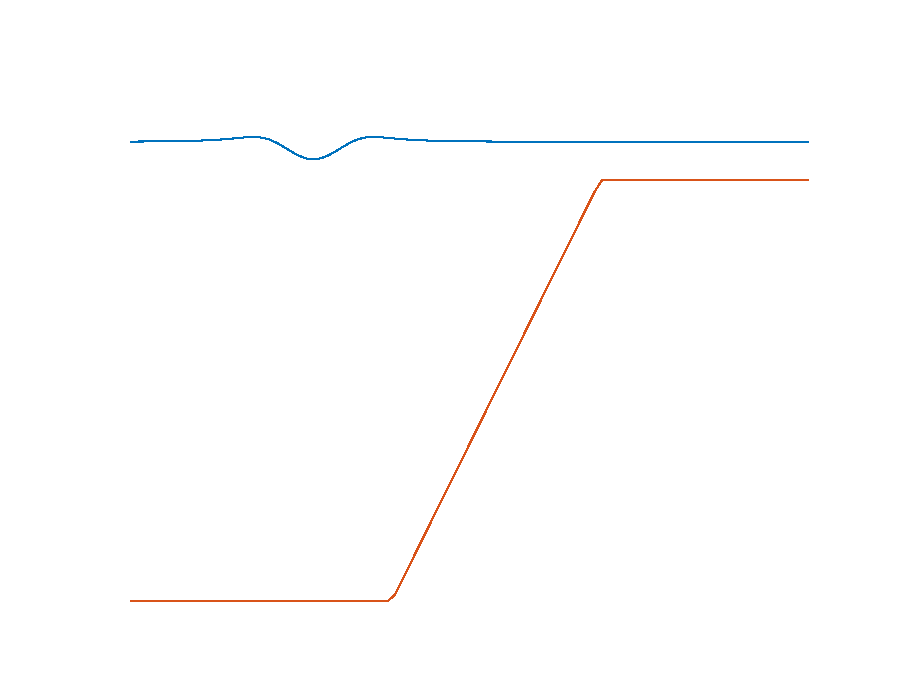
\includegraphics[width=\textwidth]{fig/2dLin1.eps}
\label{fig1}
\end{subfigure}
\begin{subfigure}[b]{0.24\textwidth}
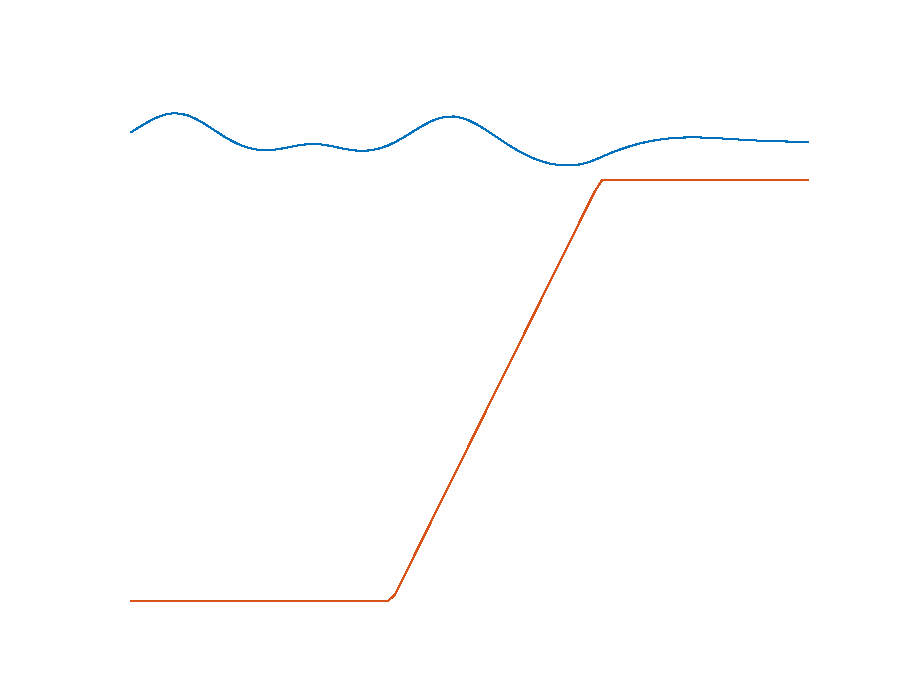
\includegraphics[width=\textwidth]{fig/2dLin2.eps}
\label{fig1}
\end{subfigure}
\begin{subfigure}[b]{0.24\textwidth}
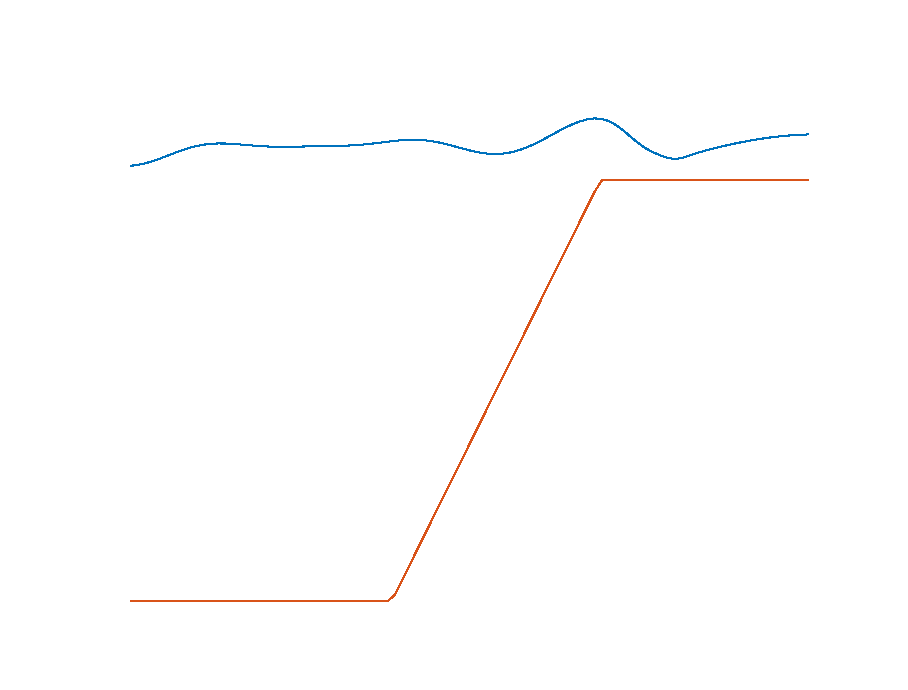
\includegraphics[width=\textwidth]{fig/2dLin3.eps}
\label{fig1}
\end{subfigure}
\begin{subfigure}[b]{0.24\textwidth}
\includegraphics[width=\textwidth]{fig/2dLin4.eps}
\label{fig1}
\end{subfigure}
\caption{Illustrating example of a 2D wave (blue) with varying seabed (red) building up as it reaches the shallow end.}
\label{fig:2dWave}
\end{figure}

\begin{figure}[!h]
\centering
\begin{subfigure}[b]{0.49\textwidth}
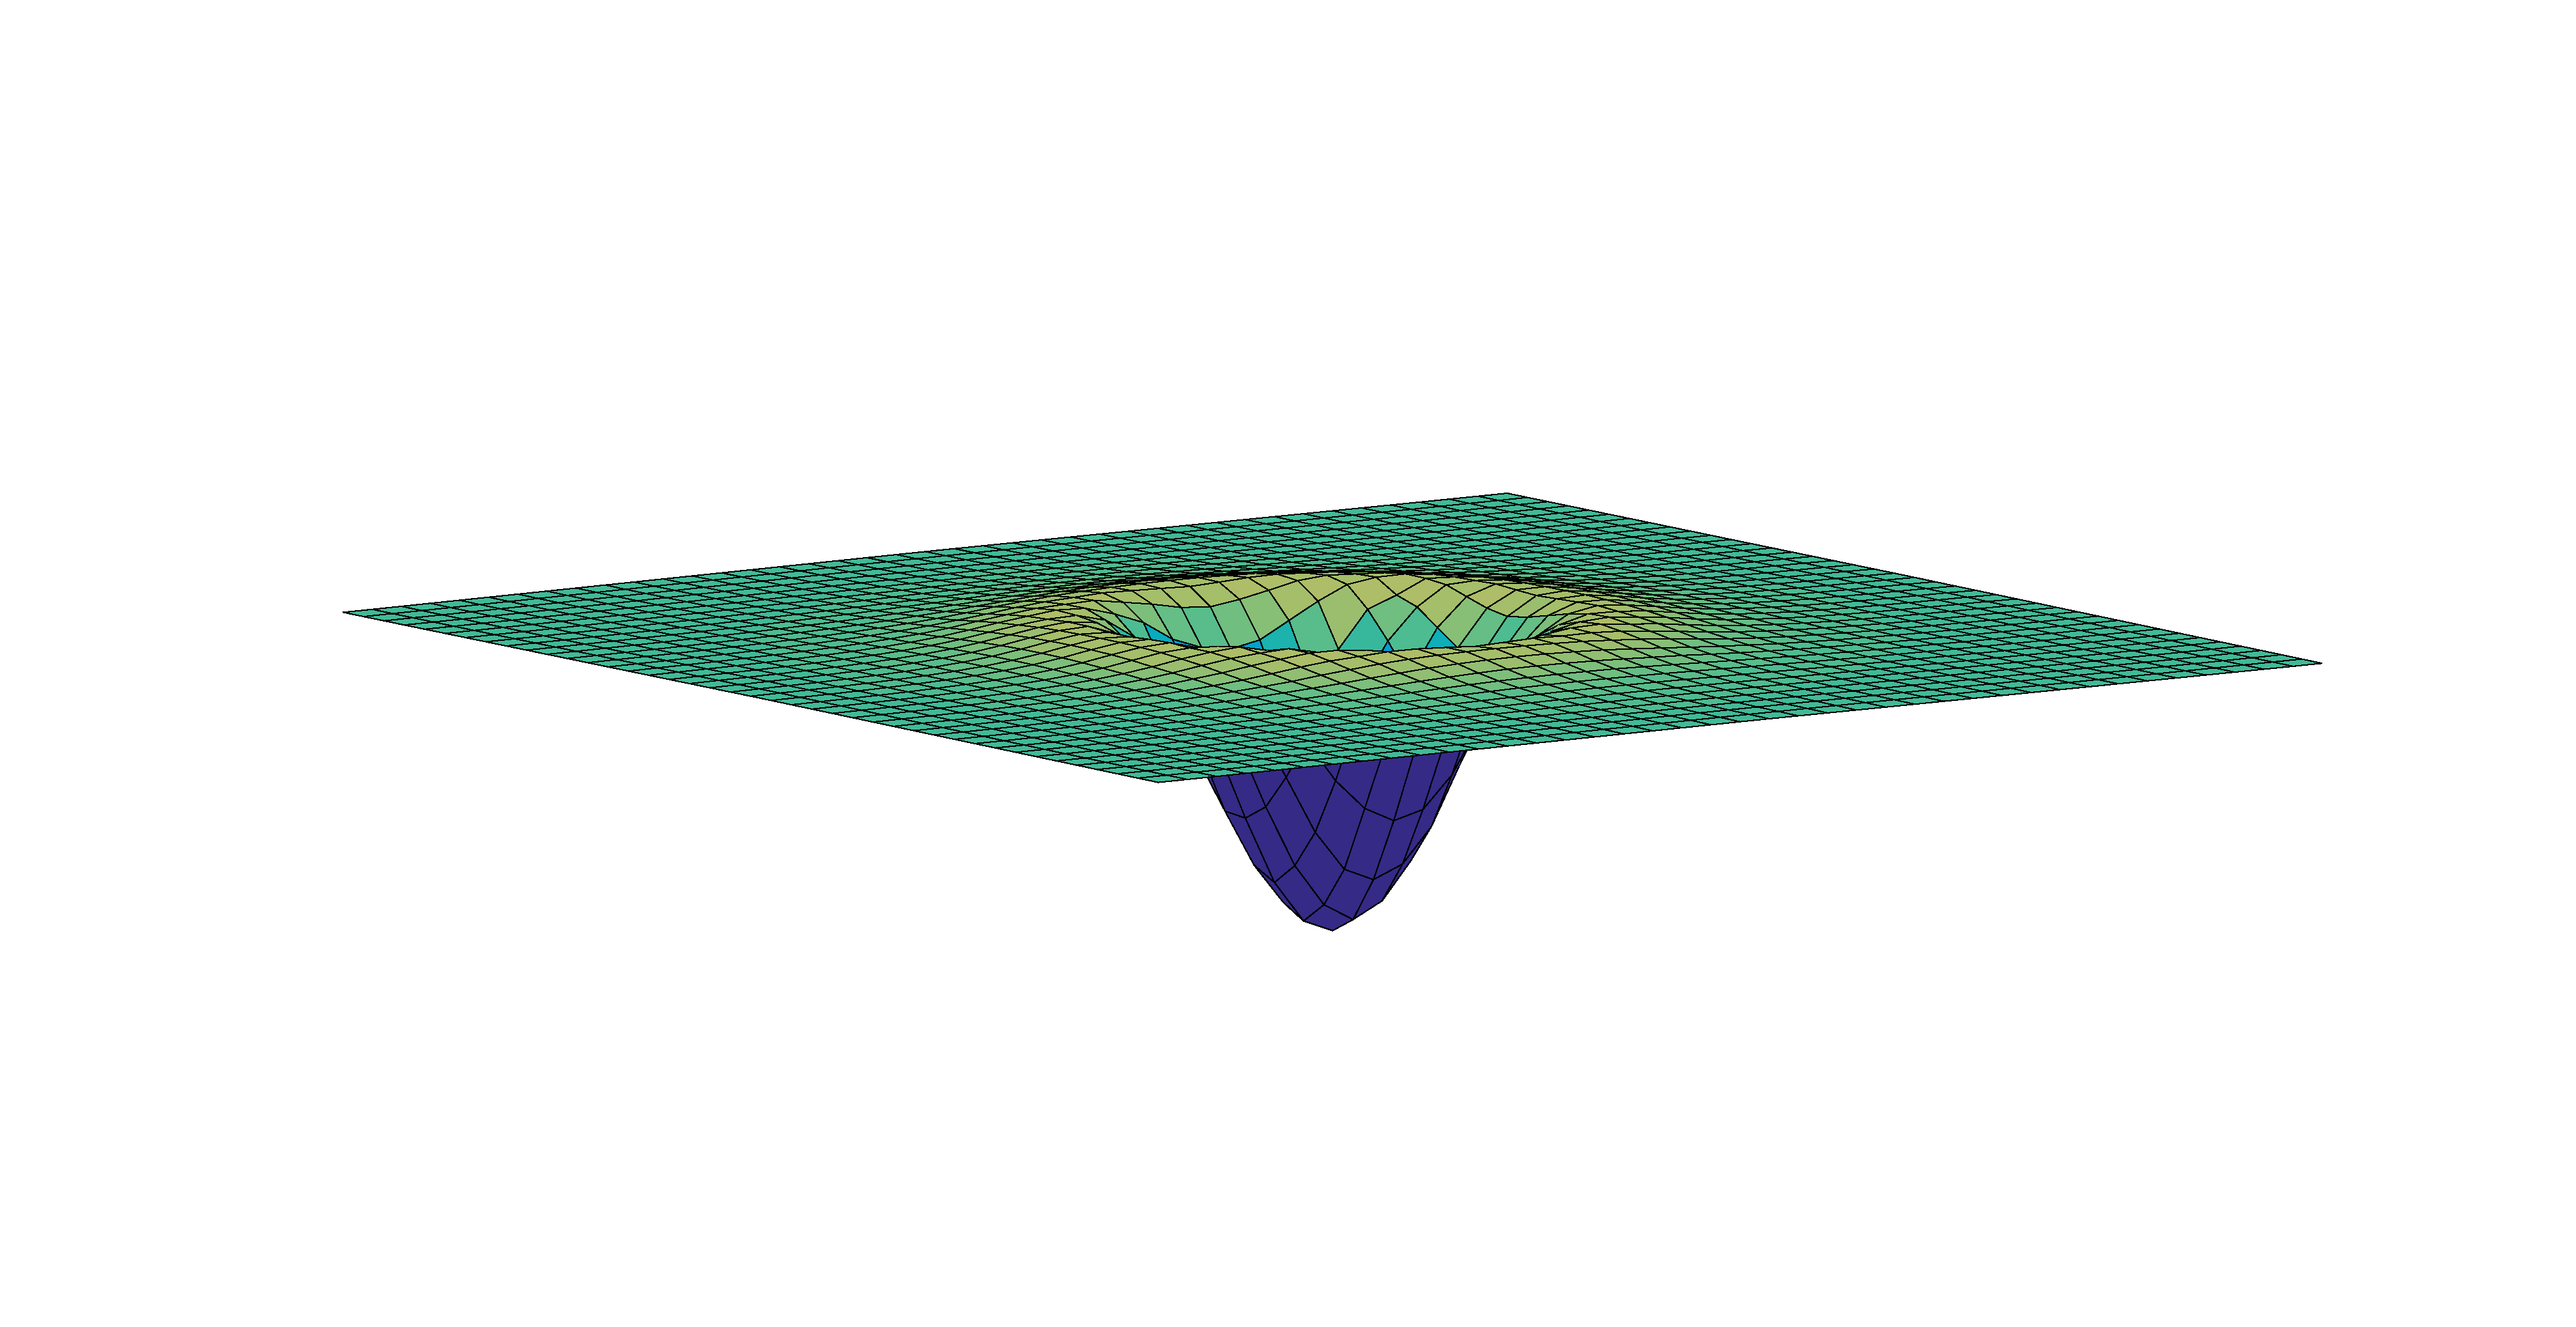
\includegraphics[width=\textwidth]{fig/3dv2_1.eps}
\label{fig1}
\end{subfigure}
\begin{subfigure}[b]{0.49\textwidth}
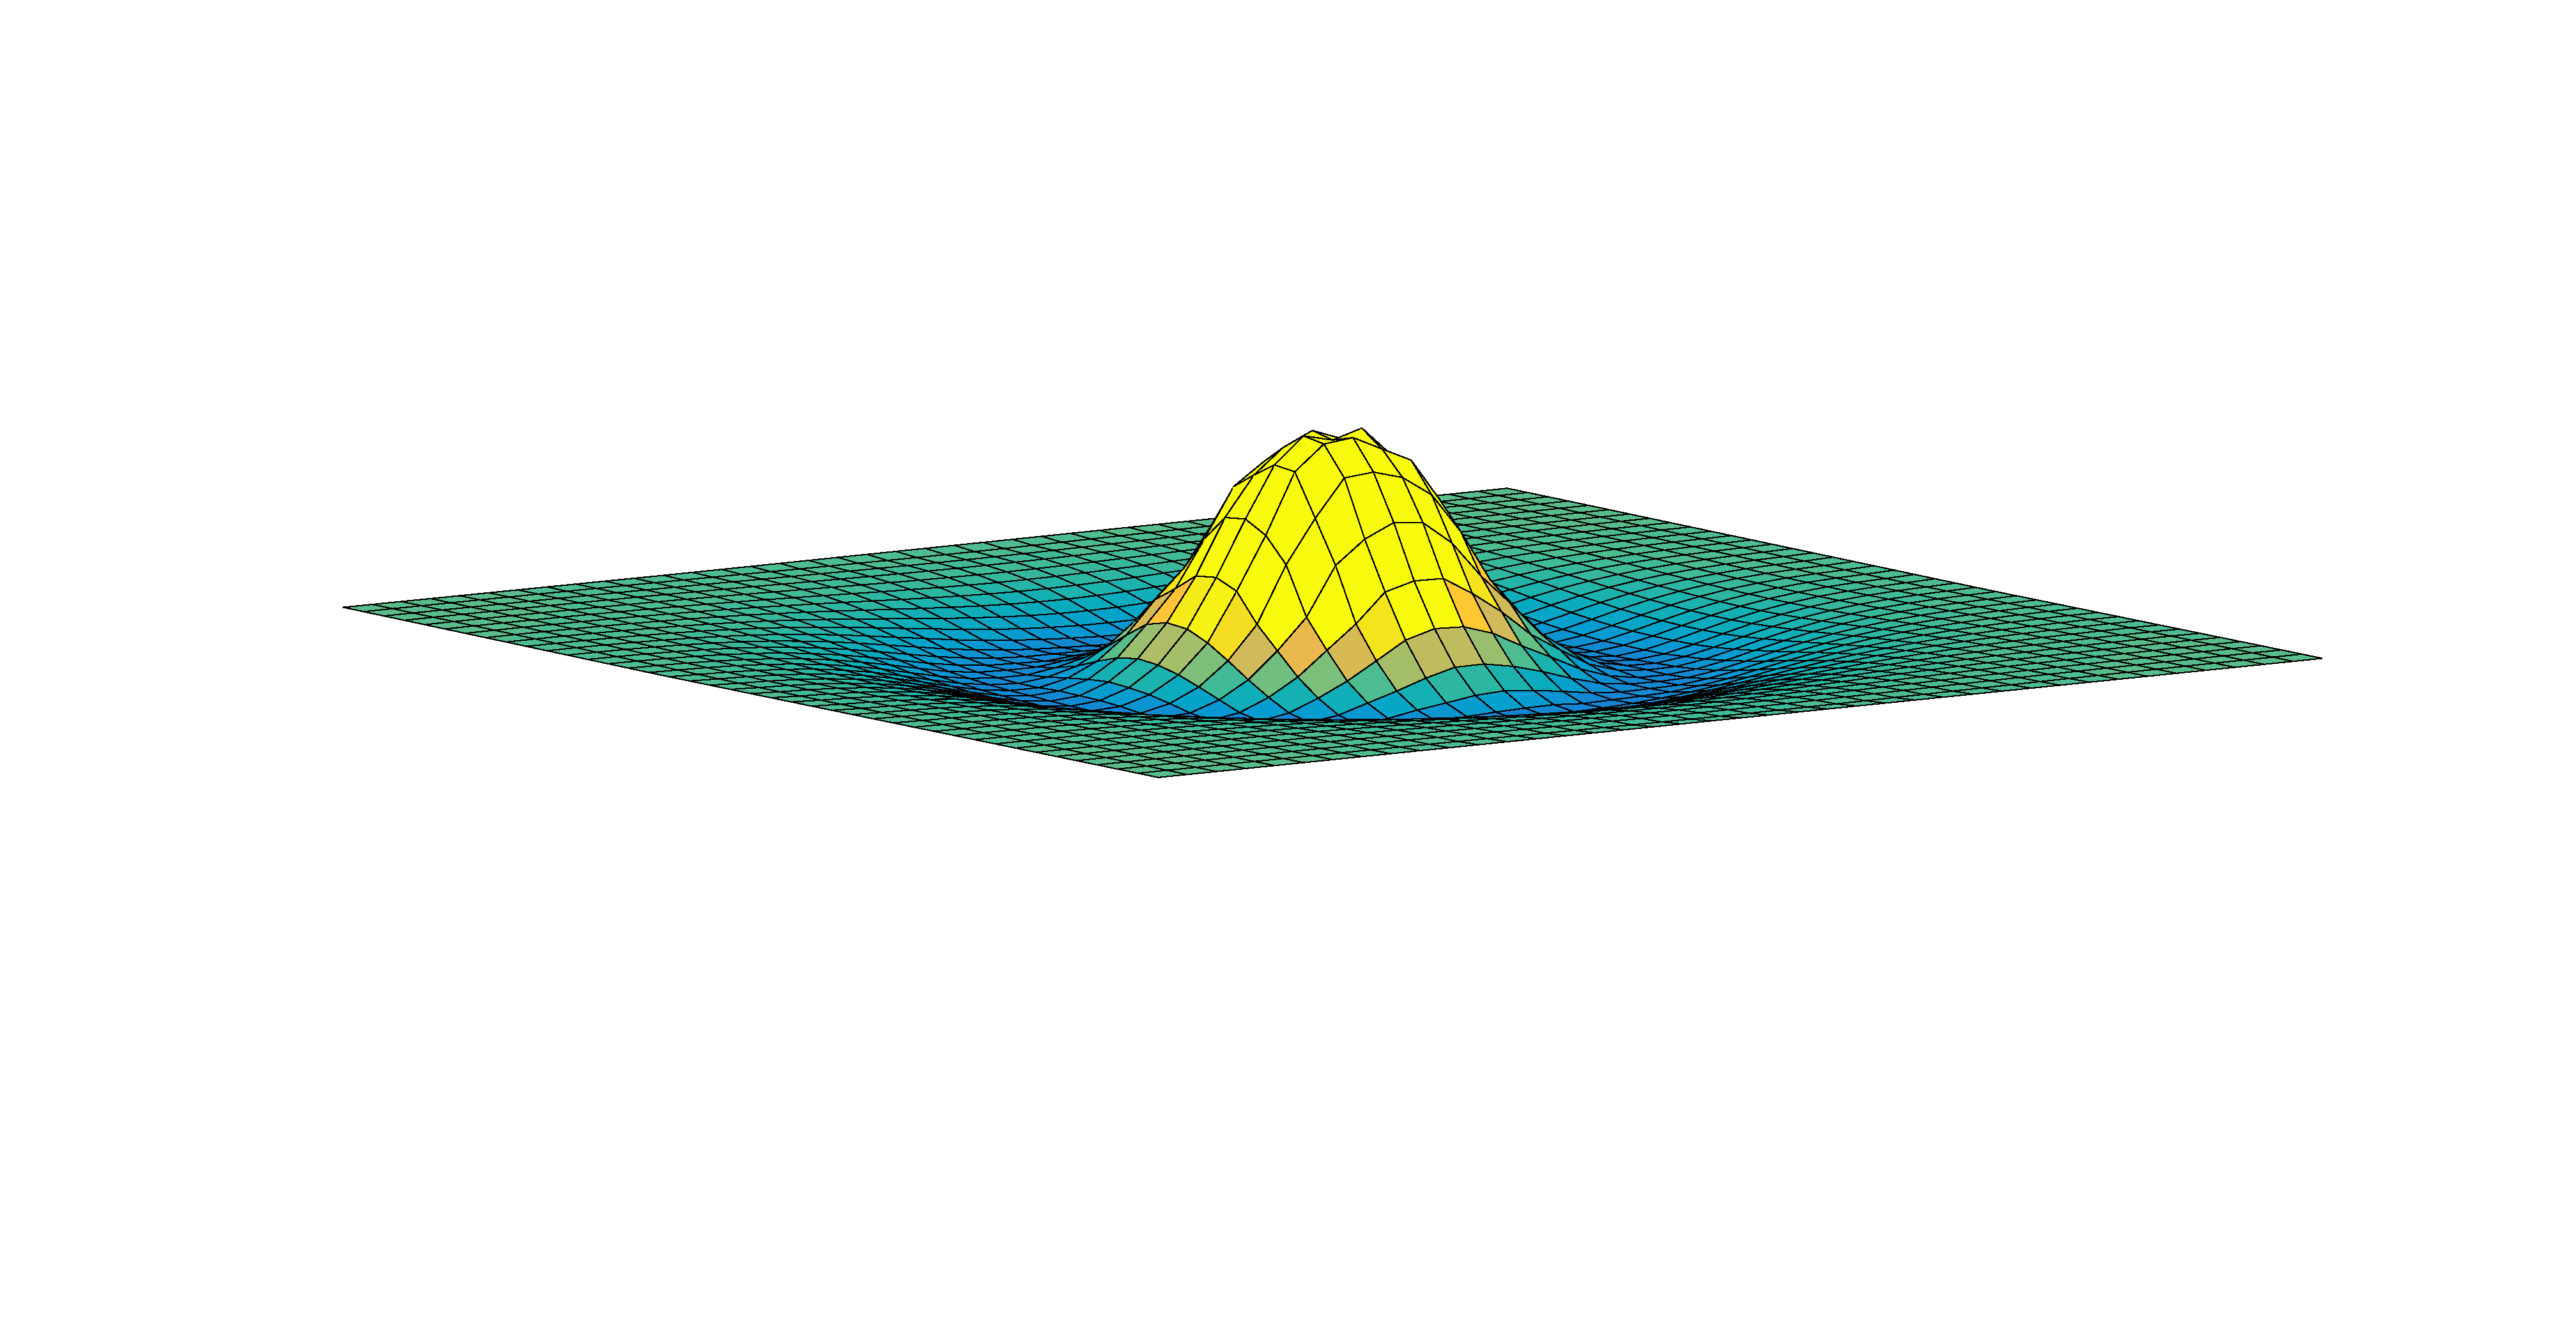
\includegraphics[width=\textwidth]{fig/3dv2_2.eps}
\label{fig1}
\end{subfigure}
\begin{subfigure}[b]{0.49\textwidth}
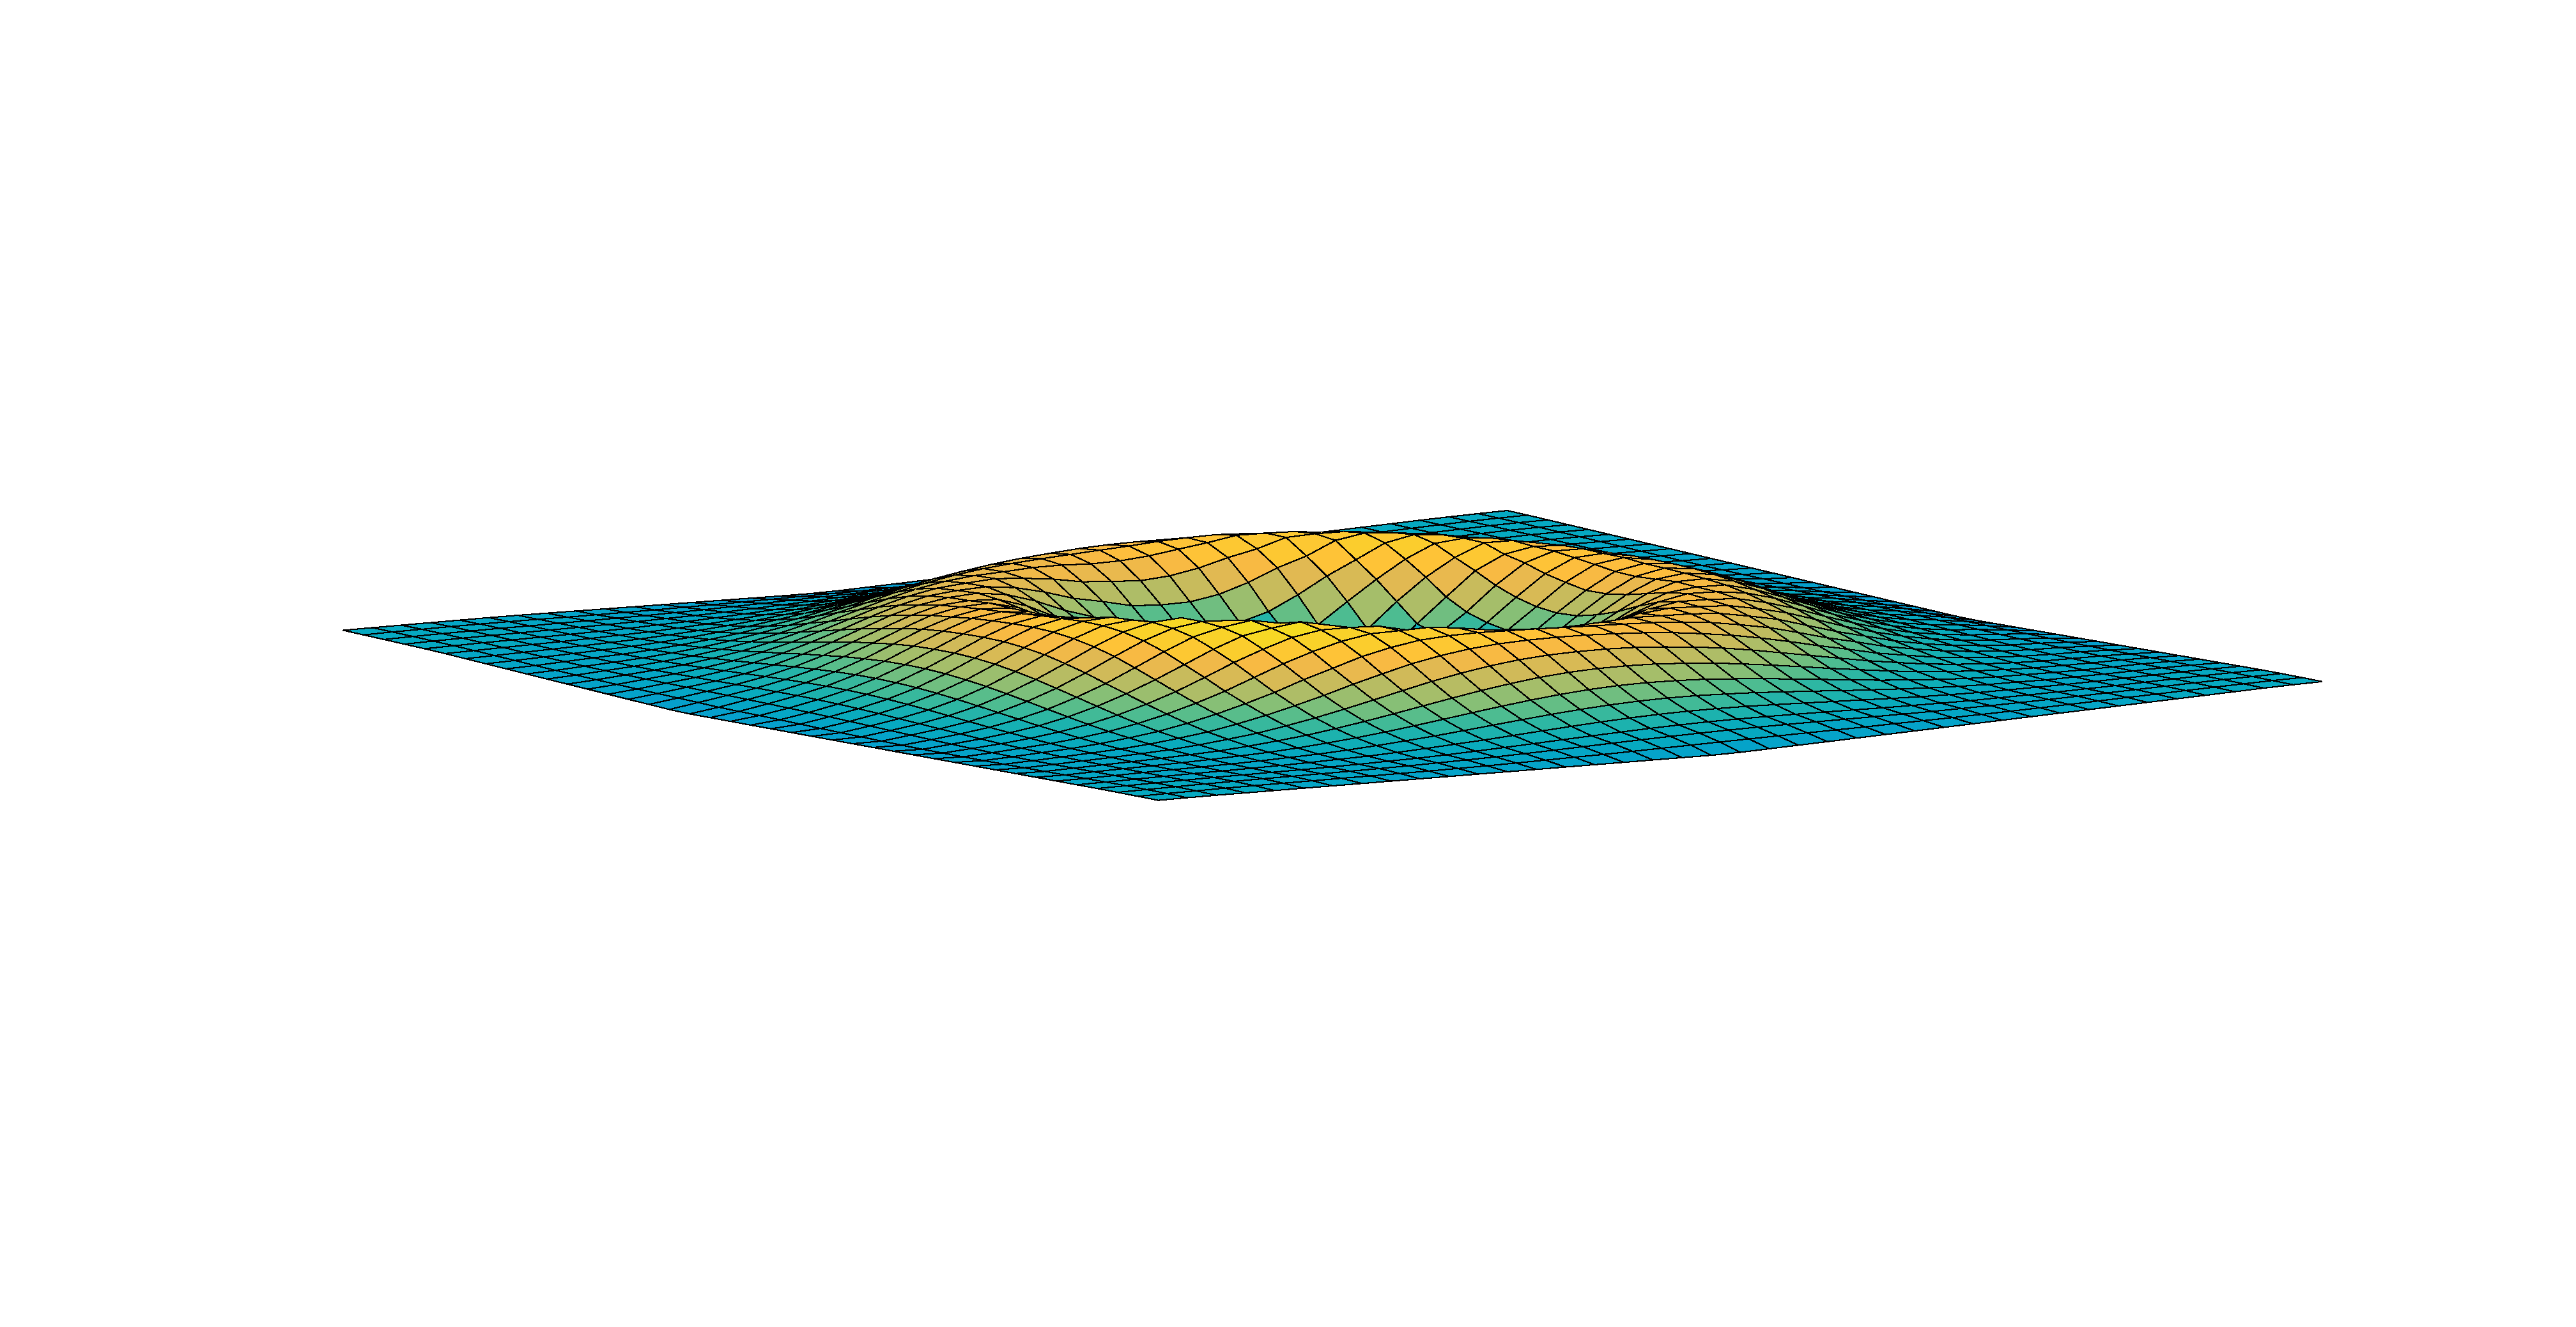
\includegraphics[width=\textwidth]{fig/3dv2_3.eps}
\label{fig1}
\end{subfigure}
\begin{subfigure}[b]{0.49\textwidth}
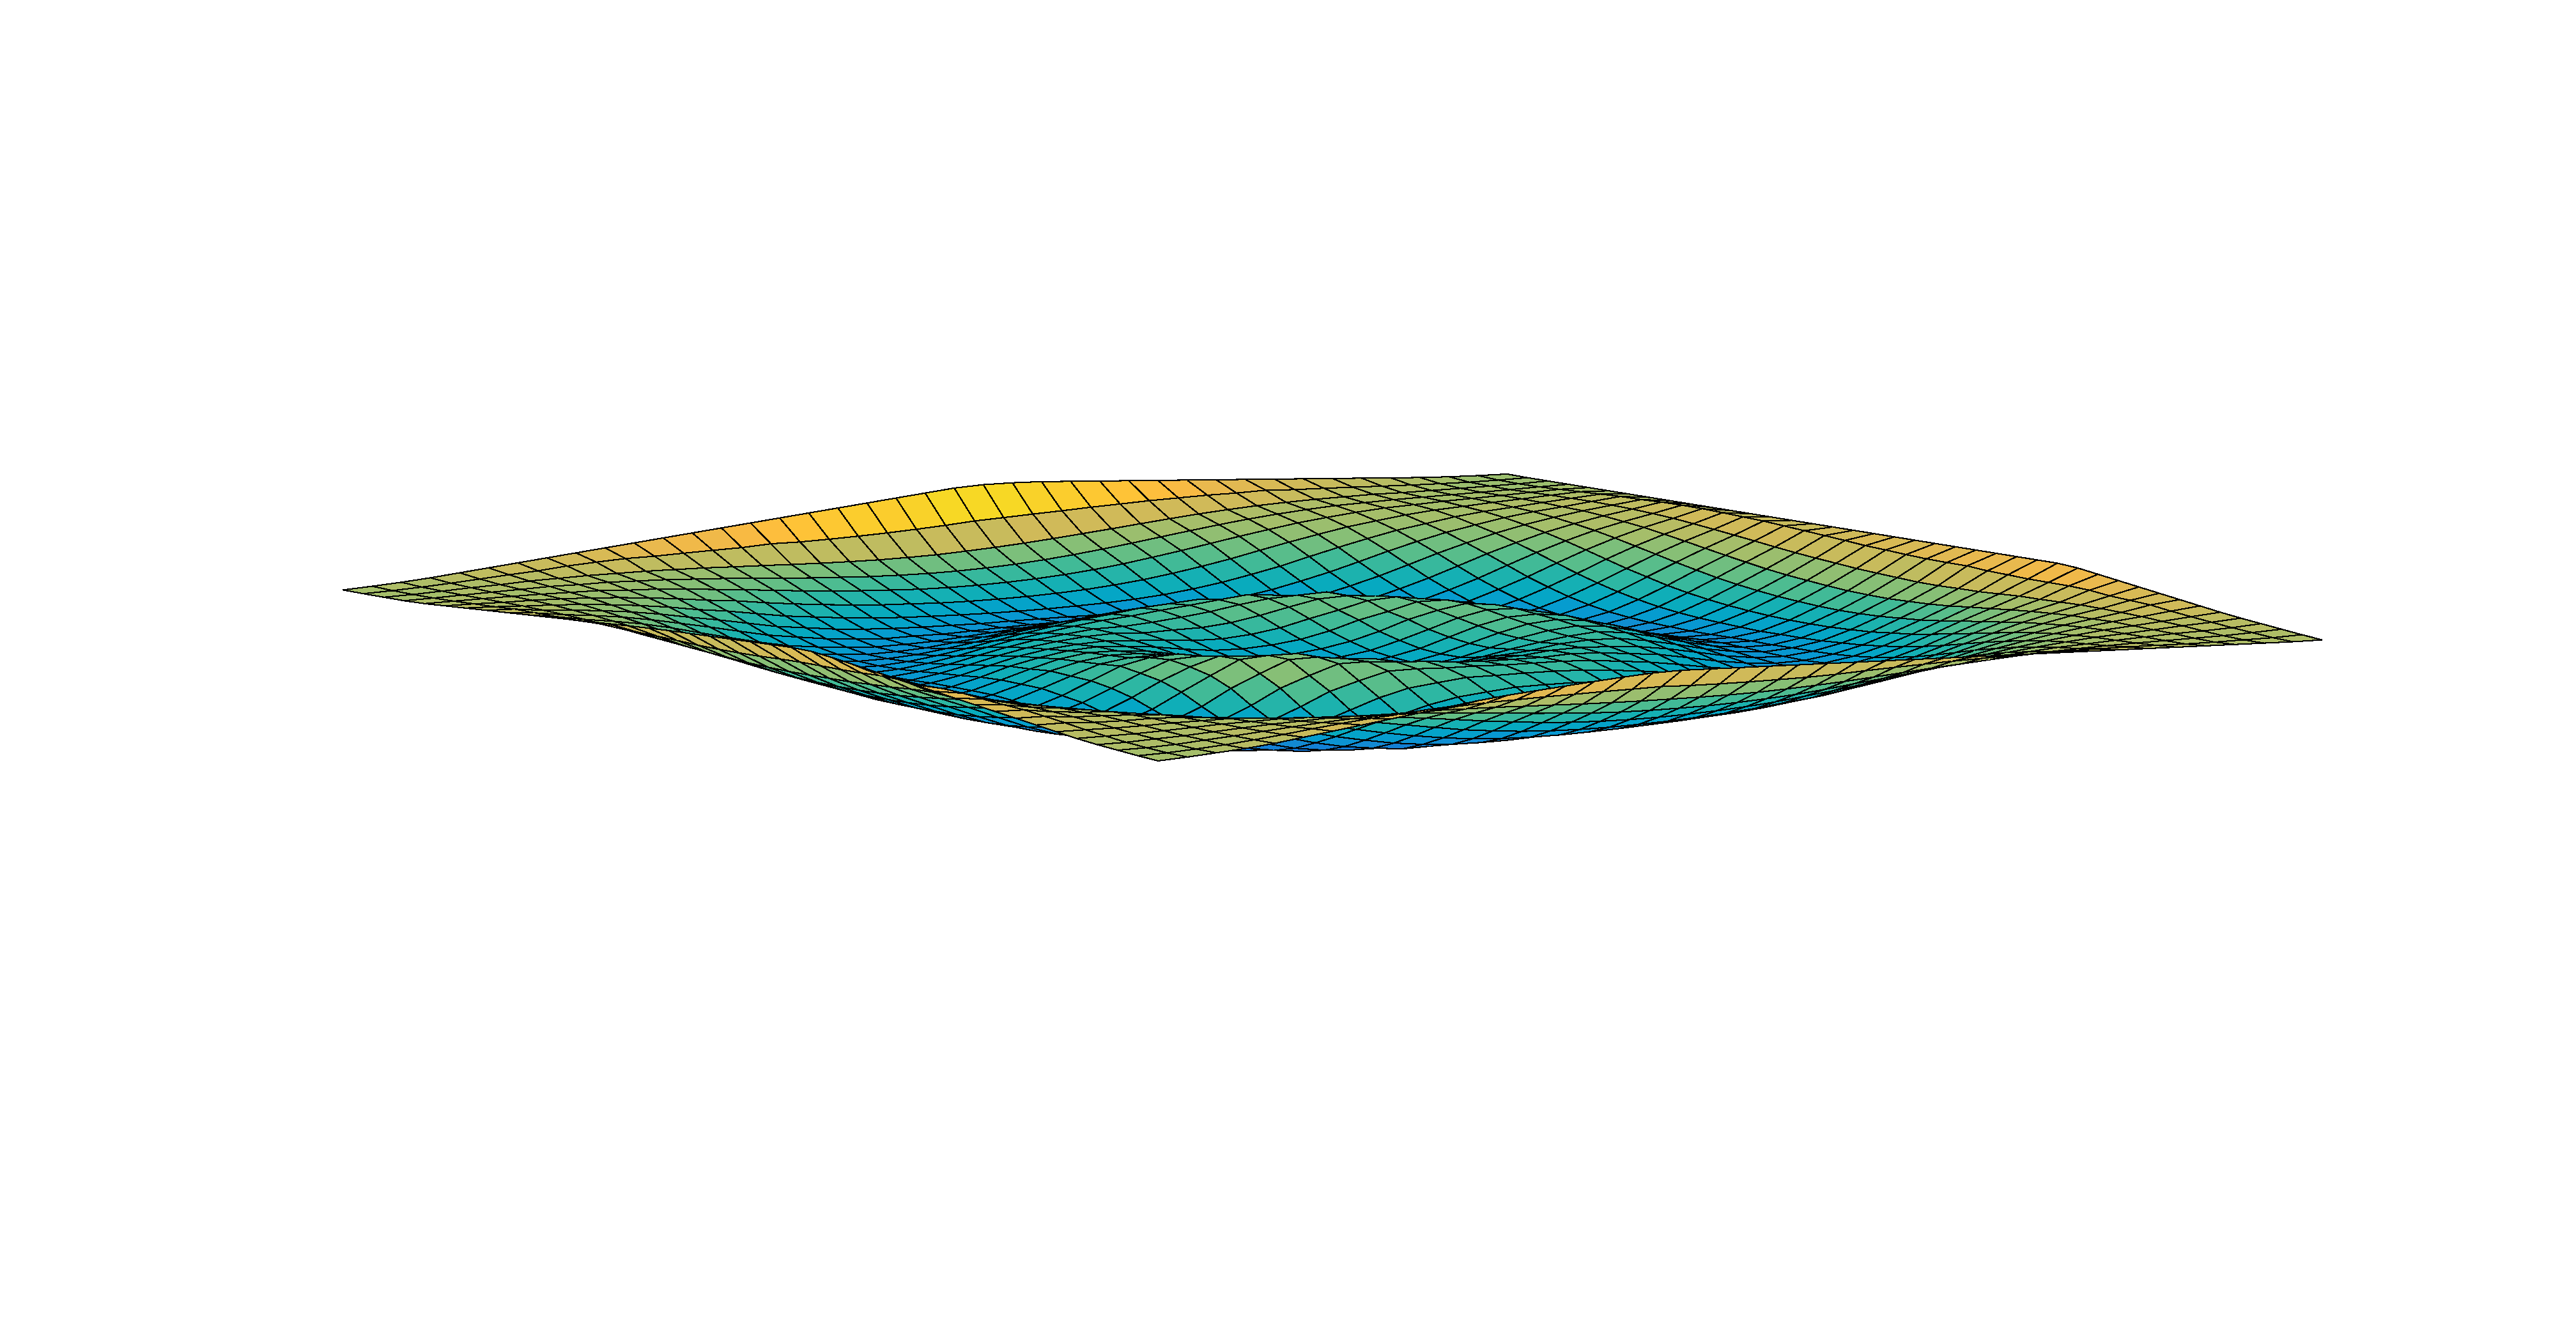
\includegraphics[width=\textwidth]{fig/3dv2_5.eps}
\label{fig1}
\end{subfigure}
\caption{Illustrating example of a 3D wave.}
\label{fig:3dWave}
\end{figure}

\clearpage

%
%    Inundation
%
\section{Inundation}
When the wave approaches the shore, the water depth becomes small. We now want to show that when the water depth is much smaller than the typical wavelength, we can estimate the situation by the following equations 
\begin{align}
u_t + \left(\frac{1}{2}\varepsilon u^2 + \eta\right)_x = 0, \label{shallow2}\\
\eta_t + (u(\varepsilon\eta + h))_x = 0 \label{shallow1}  
\end{align}
where $u = \phi_x$. \\
\\
In this section we assume the reader is familiar with scaling of variables and will not explain how this is done. To find \eqref{shallow2} we consider \eqref{eq:phiEq} and take the partial derivative with respect to $x$.
We use scales $T$ for time, $\Phi$ for $\phi$, $X$ for the $x$-direction and $Z$ for the $z$-direction. For $\eta$ we scale with $E$ and for $h$ we scale with $H$. We assume the solution is invariant in the $y$-direction
and use that $\phi_x=u$. Then we get 
\begin{equation*}
\frac{\Phi}{T}\frac{\partial u}{\partial t} + \frac{\Phi^2}{2X^2}\frac{\partial (u^2)}{\partial x}+ \frac{\Phi^2}{2Z^2}\frac{\partial(\phi_z^2)}{\partial x} + g\frac{E \partial \eta}{\partial x} = 0,
\end{equation*}
where $\partial\phi_z^2/\partial x=0$. We multiply by $T$ and divide by $\Phi$ and collect the derivatives with respect to $x$,
\begin{equation}
    \label{shallow2-ferdig}
    u_t + \left(\frac{T\Phi}{2X^2}u^2 + \frac{gTE}{\Phi}\eta\right)_x = 0.
\end{equation}
From \eqref{shallow2-ferdig} we see that $E = \frac{\Phi}{T g}$ and $\varepsilon =\frac{\Phi T}{X^2}$, and we have derived \eqref{shallow2} for scaled variables.\\
\\
Next we want to derive \eqref{shallow1}. To do this, we start with \eqref{eq:etaEq} in $z = \eta$. When scaled this is 
\begin{equation}
    \label{eta_t..}
    \eta_t + \frac{\Phi T}{X^2}\phi_x\eta_x - \frac{\Phi T}{ZE}\phi_z = 0,
\end{equation}
and see that we need an expression for $\phi_z$ in in $z = \eta$. We integrate the first equation of \eqref{eq:IncompNavierStokes} from $-h$ to $\eta$ and find 
\begin{equation*}
    \frac{1}{X^2}\phi_{xx}(E\eta + Hh) + \frac{1}{Z}\phi_z|_{z=\eta} - \frac{1}{Z}\phi_z|_{-h} = 0.
\end{equation*}
We also use from \eqref{2.9a} that in $z = -h$ we can use $\phi_z = -\phi_x\frac{n_x}{n_z} \approx -\phi_x h_x$. We now have an expression for $\phi_z$ in $z = \eta$ which is when scaled
\begin{equation*}
    \frac{1}{Z}\phi_z = - \frac{H}{X^2}\phi_x h_x - \frac{1}{X^2}\phi_{xx}(E\eta + Hh).
\end{equation*}
We insert this into \eqref{eta_t..} and get
\begin{equation} 
    \eta_t + \frac{\Phi T}{X^2}\phi_x\eta_x + \frac{T\Phi H}{EX^2}\phi_x h_x + \frac{T\Phi}{X^2}\phi_{xx}(\eta + h\frac{H}{E}) = 0.
\end{equation}
If we let $\varepsilon = \Phi T/X^2 $ as earlier and also let $\varepsilon = E/H$, then we get
\begin{equation*}
    \eta_t + (u\epsilon(\eta + h))_x = 0,
\end{equation*}
for the scaled variables, which is what we wanted to show. $\varepsilon$ turns out to be the scale of $\eta$ over the scale of $h$.  

\section{Analysis}
We are asked to compute the solutions to the following problem:
\begin{equation}
\mu \phi _{xx} + \phi_{zz} = 0
\label{eq-ana:sjefsproblemet}
\end{equation}
With boundary conditions
\begin{equation}
\phi _z = 0
\end{equation}
for $z = -1$, and
\begin{equation}
\mu \phi_{tt} + \phi_z = 0
\end{equation}
for $z = 0$.

We decide to use separation of variables:
\begin{equation}
\phi(x,z,t) = X(x)Z(z)T(t)
\end{equation}

After imposing harmonic boundaries i.e. $\phi(x) = \phi(x+L)$ ($L$ is the distance in direction $x$ in our domain of consideration)
we now that $X(x)$ must be harmonic. The same argument goes for $T(t)$. This leads us to the equation
\begin{equation}
\phi_k (x,z,t) = Z_k(z) \exp \Big( i \big( kx - \omega(k)t \big) \Big)
\end{equation}
where $k=\frac{2 \pi n}{L}$, a necessity to make $X(x) = X(x+L) = 0$. $k$ can take multiple values as a function of $n$,
all of which lead to different solution to our problem \eqref{eq-ana:sjefsproblemet}. Lets start by puting the separated $\phi$ into the primary equation.
\begin{equation}
\mu \phi_{xx} + \phi_{zz} = 0 \Longrightarrow \mu \frac{X '' (x)}{X(x)} = -\frac{Z '' (z)}{Z(z)}
\label{eq-ana:separasjon}
\end{equation}

Which must be constant as both sides of the equation are functions of different variables. Equation \eqref{eq-ana:separasjon}
leads to a second order differential equation that can be solved using characteristic equations
\begin{equation}
Z''(z) - \mu k^2 Z(z) \Longleftrightarrow r^2 - \mu k^2 = 0.
\end{equation}
Solving the characteristic equation gives us $r = \pm \sqrt{\mu}k$ meaning
\begin{equation}
Z(z) = A e^{\sqrt{\mu}k z} + Be^{-\sqrt{\mu}k z}
\end{equation}

Using the initial condition for $z = -1$ we find an expression for the constant $B$, which inserted into the expression for $Z(z)$ leads to
\begin{equation}
Z_k(z) = A_k \left( e^{\sqrt{\mu}kz} + e^{ \sqrt{\mu}k(z+2) } \right).
\end{equation}

The other initial condition (for $z=0$) makes us able to find an expression for the dispersion constant, $\omega(k)$,
\begin{equation}
\mu \phi_{tt}(x,0,t) + \phi_{z}(x,0,t) = 0 \Longleftarrow \mu \frac{T''(t)}{T(t)} = - \frac{Z'(0)}{Z(0)}.
\label{eq-ana:ini2}
\end{equation}
Solving \eqref{eq-ana:ini2} with respect to $\omega(k)$, we find
\begin{equation}
\omega(k) = \left( \frac{k}{\sqrt{\mu}} \right)^{\frac{1}{2}}
\end{equation}

We now have an expression for each solution $\phi_k(x,z,t)$,
\begin{equation}
\phi_k(x,z,t) = A_k \left( e^{\sqrt{\mu}kz} + e^{-\sqrt{\mu}k(z+2)} \right) e^{i\big( kx - \omega(k)t \big)}
\end{equation}

We may use the superposition principle to assess the solution $\phi(x,z,t)$:
\begin{equation}
\sum_{k=0}^{\infty} Z_k e^{i\big(kx - \omega(k) t \big)}
\end{equation}

\end{document}
